% \graphicspath{{./gfx/}{../figures/}{/media/data/Work/cnstellate/}{/media/data/Work/cnstellate/TV_Notch/}{/media/data/Work/Responses/}{/media/data/Work/thesis/ans2010/gfx/}}

\section[TV Cell Model]{Tuberculoventral cell model: Optimisation to notch-noise response \label{sec:TV-cell-model}}
% - A
% ------------------------------------------------------------------------------

\subsection{Background}

\TV~or vertical cells are glycinergic, inhibitory cells found in the deep layers of the \DCN~that send axon collaterals to the \VCN\@.
They are characterized as having a non-monotonic response to tones with increasing sound level and respond poorly to broadband noise \citep{SpirouDavisEtAl:1999,NelkenYoung:1997,ReissYoung:2005}, as shown in Fig.~\ref{fig:SpirouFig1}.
Anterograde labeling in the \DCN~suggests \TV~cells project tonotopically to the \VCN~not just on-CF, but also to the low and high frequency side bands \citep{MunirathinamOstapoffEtAl:2004,OstapoffMorestEtAl:1999}.
Ultra-structural labeling of synapses in the rat \DCN~suggest \TV~cells are inhibited by glycinergic \DS~cells and from sources in the \DCN~but excitatory inputs were not found from \TS~cells in the rat \citep{Rubio:2005}.
Evidence in the mouse suggests otherwise since intracellular responses from labeled \TV~cells in the mouse show clear excitatory input from \TS~cells and diffuse inhibitory input from \DS~cells \citep{ZhangOertel:1993b,WickesbergOertel:1993}.

%\smallskip{}

TV receive mono-synaptic excitatory input from auditory nerve fibers \citep{OertelWu:1989,ZhangOertel:1993b}.
Taken together, these two results suggest that \LSR~auditory nerve fibers may form the major excitatory input to type~II cells.
If true, this hypothesis could also explain the finding that type II units have consistently higher thresholds than \DCN~principal cells \citep{YoungBrownell:1976} because \LSR~auditory nerve fibers also have elevated thresholds relative to the lowest threshold auditory nerve fibers \citep{Liberman:1978}.
However, patterns of auditory nerve innervation of the \DCN~are most consistent with \HSR~fiber innervation of \TV~cell somata and \LSR~fiber innervation of dendrites \citep{Liberman:1993}.
In that case, the low spontaneous rates and high sound thresholds of type II units might be caused by a high intrinsic electrical threshold \citep{HancockDavisEtAl:1997}; this is consistent with the responses of vertical cells to intracellular current injection \citep{DingVoigt:1997,ZhangOertel:1993b}.

%\smallskip{}

Type~II units also supply an inhibitory input to the \VCN~\citep{WickesbergOertel:1990}, but the role of type~II terminals in the \VCN~is less clear.
Three different hypotheses have been raised.
The first is that this projection modulates the response thresholds of \VCN~neurons \citep{PaoliniClark:1998}.
The role of type~II units in spectral processing is that of a narrowband inhibitor. Responses of \DCN~principal cells are strongly inhibited by this narrowband source.
As a result, \DCN~principal cells are inhibited by sharp spectral peaks close to their \BF~\citep{SpirouDavisEtAl:1999}.

%\smallskip{}

\begin{figure}[htb]
  \centering
  % \resizebox{5in}{!}{\includegraphics[angle=-90]{NoFigure}}
  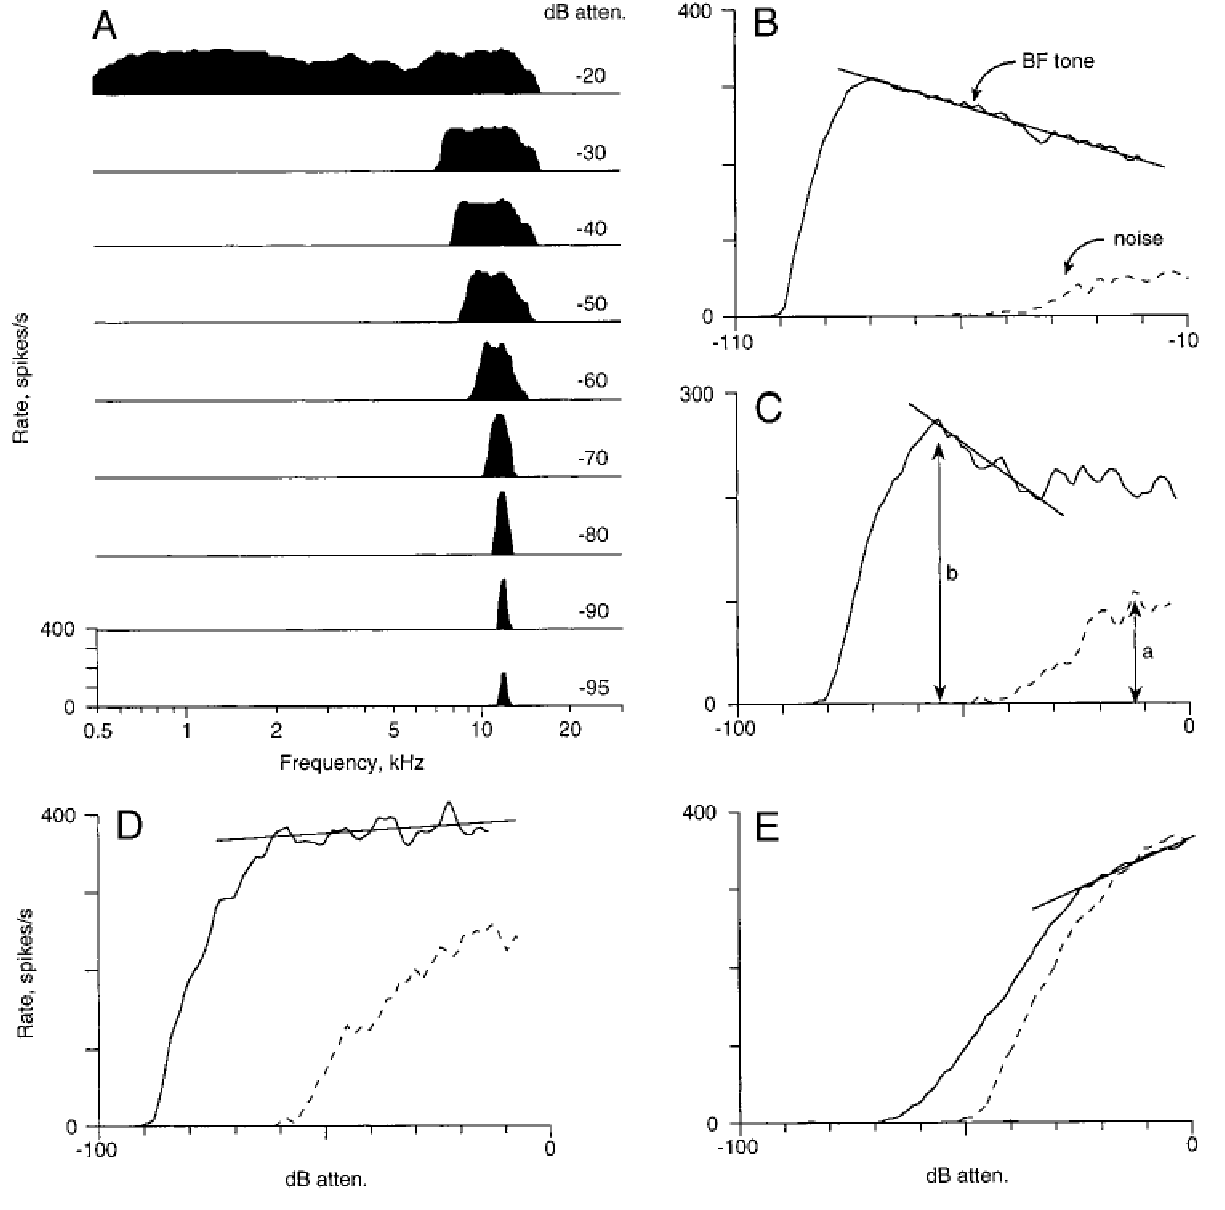
\includegraphics[keepaspectratio,width=0.8\textwidth]{Spirou-Fig1-type2}
  \caption[Experimental data of a single Type-II~DCN~unit]{Experimental data of a single Type-II~DCN~unit \citep[Fig.~1]{SpirouDavisEtAl:1999}.}   \label{fig:SpirouFig1}
\end{figure}\yellownote{Figure~\ref{fig:SpirouFig1} needs permission}


\subsubsection{Modeling of Tuberculoventral cells}

\yellownote{Expand previous studies  of the DCN incl. TV cells}


\citet{ArleKim:1991a} were the first to show type~II \EIRA~with simple McCullock-Pitts point neuron models.


{\it (From Hancock Davis Voigt 97) Blum et al. (1995) used a wideband inhibitory   mechanism to create type II unit responses in a model of the DCN. In that   model, each cell population was described by a mathematical formula for its   steady-state rate-level function. This level of abstraction was used to focus   specifically on the role of network connectivity in determining the   steady-state behavior of DCN units. The level of abstraction employed in our   model allows for examination of temporal response properties including PST   histograms and cross-correlation analysis.}

\citep{DunnVetterEtAl:1996} performed some modelling.


Modeling of Type~II units in the \DCN~has been thoroughly categorised by Kevin Davis and colleagues \citep{YoungDavis:2002,HancockDavisEtAl:2001,DavisYoung:2000,SpirouDavisEtAl:1999,HancockDavisEtAl:1997,DavisVoigt:1996,DavisVoigt:1994,DavisVoigt:1991}.
 Low spontaneous rate is created in a neural model by either increasing the intrinsic spiking threshold or lowering the synaptic strength of the inputs.
Intracellular observations in decerebrate gerbils show higher thresholds in type~II units \citep{DingVoigt:1997}; and observations of hyperpolarisation responses to off \gls{BF}~tones in intracellularlly recorded type II units.
 
Another case for type II behaviour of no spontaneous activity, is a preference of \LSR, high threshold \AN~fibres over \HSR~fibres to synapse with \TV~cells.
Whether \LSR~fibres preference the deep layers of the \CN~are yet to be confirmed \citep{Ryugo:2008,MeltzerRyugo:2006,RyugoParks:2003,BabalianJacommeEtAl:2002}.

%\smallskip{}

\citep{Rhode:1999} Vertical cells in gerbils (mainly type III)

%\smallskip{}

The intrinsic mechanism is more favourable in Type II units, provided there is sufficient inhibition and excitation \citep{HancockDavisEtAl:1997}.
Lateral inhibition was disregarded in favour of wide-band inhibition \citep{HancockDavisEtAl:1997}.
 %\smallskip{}

Work by Reed and Blum \citep{ReedBlum:1995,BlumReedEtAl:1995,ReedBlum:1997,BlumReed:1998} on the circuitry of the \DCN~showed that wide-band inhibition was necessary for the principal cells of the \DCN~including type II units.
 %\smallskip{}

With retrograde labelling in the \DCN~three types of ventro-tubercular units in rats were identified \citet{FriedlandPongstapornEtAl:2003}, as apposed to only two types in cats \citep{SmithRhode:1989,OertelWuEtAl:1990}.
These units are identified as \TS~and \DS~cells, with the third in rats identified as small adendritic neurons.

\yellownote{The above paragraphs need to be cleaned up and worked into the idea of generating BNN models using a simple approach} 
%\smallskip{}

% \subsubsection{Key design factors}


% \textbf{Morphological}
% \begin{itemize}
% \item vertical/multipolar cell in deep layer of \DCN~\citep{Rhode:1999}
% \item receive small number of \ANF~syn to dend
% \item receive large number of Gly and \GABA~syn to soma and dendrite
% \end{itemize}





% \begin{itemize}
% \item Rat model (no \TS-TV) but has been shown in other mammals
% \item Unable to include other \DCN~inputs
% \item Model must show \DSTV~inhibition and offset of distribution

% \item Notch noise stimulus $\rightarrow$ need more \TV~cells across frequency
% \item Input \SPL~and weight of excitation affect spiking output
% \item Larger network $\rightarrow$ increased computational load
% \item Solution: Parallelism model
% \end{itemize}

The notch sweep sets used by \citeauthor{ReissYoung:2005} were generated with logarithmically constant notch widths and notch center frequencies ranging from 1 octave below to 1 octave above \BF~in $1/50$ octave steps.

\subsection{Implementation}

The experimental data by \citet{ReissYoung:2005} was recorded from adult cats, with the notch noise produced in the frequency domain (accounting for calibration of the ear canal speaker spectrum) and sampled with fixed random phases in the time domain.
The notch noise presented in this optimisation routine was generated in Octave using frozen Gaussian noise (100kHz sampling rate) and a Chebyshev type II band reject filter.

%\smallskip{}

The experimental data, shown in Fig.~\ref{fig:TVReissFig9}, is the average responses of type II units to notch sweeps.
The optimisation routine would be prohibitive if it was a notch sweep simulated on a single neuron; therefore, this optimisation uses a single notch presentation across an entire network of TV cells.
Accordingly, the fitness function must take into account the relative position of cells in the network when comparing the experimental data.
For example, when presented with a notch noise filtered between 5kHz and 10kHz, a unit with \CF~of 5kHz will see a falling edge of a 1 octave notch, whereas a unit with \CF~of 10kHz, will see a rising edge of a half octave notch.
Figure~\ref{fig:TVNotchDiagram} shows the combination of the type II unit notch data for 1 octave.

 %\smallskip{} 
The sound level in the \citet{ReissYoung:2005} data further complicates the situation.
The power spectrum is maintained at a constant level per frequency band (dB per Hz$^2$) and this is processed and scaled at each point in the notch sweep.
For a single presentation used in this experiment the sound level plays an important part in stimulating the \ANFs~and contributing interneurons.
The experimental data shown in Fig.~\ref{fig:TVReissFig9}, show the mean response to notch sweeps at 22 dB/Hz$^{1/2}$.

%\smallskip{}

Higher thresholds in type~II \DCN~units \citep{SpirouDavisEtAl:1999} and the presence of multiple inhibitory synapses \citep{Alibardi:2006} suggest \TV~cells either receive a strong inhibitory influence or they have a lower \RMP~due to a lower leak current reversal potential. A reduced resting membrane potential may increase the threshold for excitatory inputs to generate action potentials.

% \yellownote{I allowed HSR2TV weight value go negative to give a constant  inhibitory input. Then on 2 other runs I shifted the reversal potential of the leak current to -70 and -75.}

%\smallskip{}

The big issue with the optimisation of population mean rate responses is that the model could be over simplified and remove timing information.
The \HSR~rate response is generally flat at medium to high sound intensities. 
\DS~cell response has a regular onset spike but has a low rate throughout the stimulus, which detracts from the purpose of using a whole network to optimise parameters for synaptic inputs regarding \TV~cells.
The \TV~rate response could therefore just be modeled on the \LSR~response using a simple gradient-decent method. 
\yellownote{Population mean rate: Pros: fairly stable for smallish   repetitions, Cons: removes timing}
 
%\smallskip{}


\begin{figure}[htb]
  \centering \resizebox{0.8\textwidth}{!}{\includegraphics[angle=-90]{NoFigure}}
  % \includegraphics[keepaspectratio,width=0.8\textwidth]{./gfx/TV_Reiss}
  \caption[Experimental notch-noise data of a single Type-II DCN unit]{Experimental notch-noise data of a single Type-II DCN unit \citep[,~Fig.~9]{ReissYoung:2005}.}
  \label{fig:TVReissFig9}
\end{figure}\yellownote{Permission needed for Reiss and Young figures}


\begin{figure}[htb]
  \centering \resizebox{0.6\textwidth}{!}{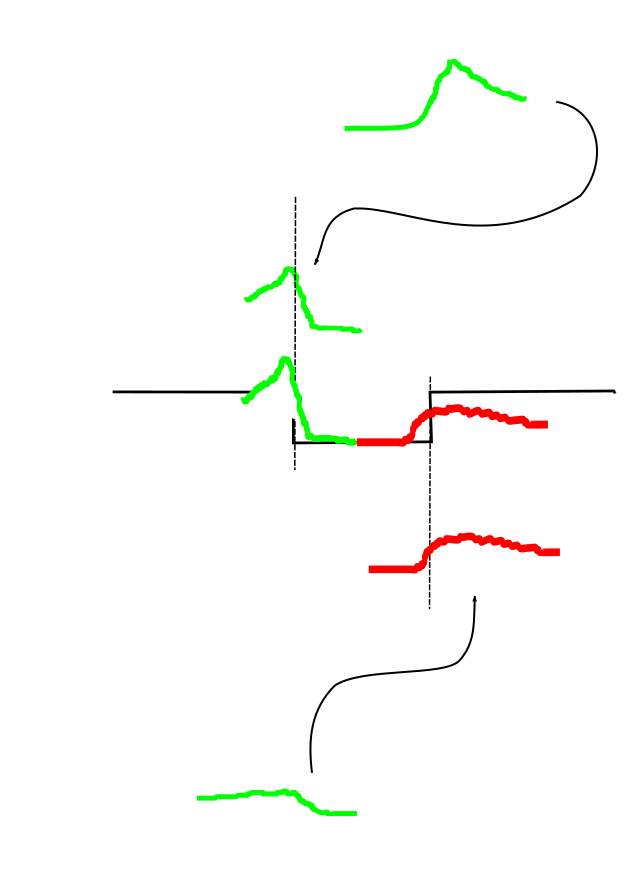
\includegraphics{TV_NotchDataConfig}}
  \caption[TV model optimisation configuration]{Expected mean rate response to notch noise in the TV cells is created from 1 octave notch sweeps (top) for the falling edge and from half octave notch sweeps (bottom) for the rising edge. (Top and bottom figures from Fig.~9 \citep*{ReissYoung:2005})}   \label{fig:TVNotchDiagram}
\end{figure}

% {
\small\linespread{0.5}
\begin{table}[htb]
    \caption{Tuberculoventral cell model summary}
    \label{tab:TVNotchModelSummary}
\end{table}
\noindent%
\begin{tabularx}{\textwidth}{|l|X|}\hline %
\hdr{2}{A}{Model Summary}\\\hline
         \textbf{Populations}          & HSR and LSR ANFs, Golgi, DS, and TV cells \\\hline
          \textbf{Topology}            & Tono-topicity of the rat AN and CN \\\hline
        \textbf{Connectivity}          & ANF$\to$\{GLG, DS, TV\}, GLG$\to$DS, DS$\to$TV  \\\hline
         \textbf{Input model}          & ANF~model: Instantaneous-rate Poisson neural model \citep{ZilanyBruce:2007} \\ \hline
\multirow{3}{*}{\textbf{Neuron model}} & GLG: Instantaneous-rate Poisson neural model\\
                                       & DS: HH-like single-compartment model (Type I-II \RM model)\\ 
                                       & TV: HH-like single-compartment model (Type I-classic \RM model) \\\hline
       \textbf{Channel models}         & $I_{\textrm{Na}}$, $I_{\textrm{KHT}}$, $I_{\textrm{KLT}}$, $I_{\textrm{KA}}$ and $I_{\textrm{h}}$ \citep{RothmanManis:2003b}\\\hline
\multirow{2}{*}{\textbf{Synapse model}} & Excitatory: AMPA glutamatergic receptor (single-exponential)\\
&  Inhibitory: \GABAa GABAergic receptor (double-exponential), Glycinergic receptor (double-exponential) \\\hline
%            \textbf{Input}             & Notch-noise stimulus \\\hline
%\textbf{Optimisation}    & Parameters for \GLGDS are optimised based on experimental click recovery date from \citet{BackoffPalombiEtAl:1997}. The praxis method is used for optimisation.  \\\hline
%\textbf{Measurements}    &  Spikes of TV units recorded and PSTH genereated. First spike latency, mean rate and variance of TV units calculated. Fitting data was compared against experimental data of a Type II~\DCN~unit~\citep[Figure~9]{ReissYoung:2005}.\\\hline
\end{tabularx}
\vspace{1ex}

% - B -----------------------------------------------------------------------------
\noindent%
\begin{tabularx}{\textwidth}{|l|X|X|}\hline
\hdr{3}{B}{Populations}\\\hline
\textbf{Name} &    \textbf{Elements}    & \textbf{Size} \\\hline
     HSR      &    Poisson generator    & $N_{\text{HSR}} = 50$ per freq.\ channel \\\hline
     LSR      &    Poisson generator    & $N_{\text{LSR}}= 30$  per freq.\ channel \\\hline
     GLG      &    Poisson generator    & $N_{\text{GLG}}= 1$  per freq.\ channel  \\\hline
     DS       &   Type I-II \RM model    & $N_{\text{DS}}= 1$ per freq.\ channel \\\hline
     TV       & Type I-classic \RM model & $N_{\text{TV}}= 1$ per freq.\ channel\\\hline
\end{tabularx}
\vspace{1ex}

% - C ------------------------------------------------------------------------------
\noindent%
\begin{tabularx}{\textwidth}{|l|l|l|X|}\hline
\hdr{4}{C}{Connectivity}\\\hline
\textbf{Name}  & \textbf{Source} & \textbf{Target} & \textbf{Pattern} \\\hline
%   ANF$\to$DS &       ANF       &   D~Stellate    & Skewed Gaussian, centered at CF, spread below CF \sANFDSl, spread above CF \sANFDSh \\\hline
    \ANFTV     &    LSR, HSR     &       TV        & 
Narrowband connection on CF, zero spread, weight \wLSRTV and \wHSRTV, number \nLSRTV and \nHSRTV, delay \dANFTV \\\hline
%   GLG$\to$DS &      Golgi      &   D~Stellate    & Gaussian, centered at CF with spread \sGLGDS \\\hline
    \DSTV      &       DS        &       TV        & 
Gaussian convergence, centered on CF, spread \protect{$\sigma^2 = \sGLGDS$}, weight \wGLGDS, number \nGLGDS, delay $\dGLGDS=0.5$ ms \\\hline
\multicolumn{4}{|>{\centering}X|}{\ANFGLG, \ANFDS, and \GLGDS from Table~\ref{tab:TVModelSummary} }\\\hline
\end{tabularx}
% , uniform weight \wANFDS for all synapses, number \nLSRDS \& \nHSRDS, delay \dANFDS
\vspace{1ex}

% - D ------------------------------------------------------------------------------
\noindent%
\begin{tabularx}{\textwidth}{|l|X|}\hline
\hdr{2}{D}{Neuron and Synapse Model}\\\hline
        \textbf{Name}          & TV cell model \\\hline
        \textbf{Type}          & Type I-classic \RM model \citep{RothmanManis:2003b}, conductance synapse input \\\hline
\textbf{Subthreshold dynamics} & Na, KHT, Ih, and leak currents \\\hline
       \textbf{Spiking}        & Emit spike when $v(t) \geq \theta$  \\\hline
\end{tabularx}
\vspace{1ex}
% \noindent\begin{tabularx}{\textwidth}{|p{0.150.95\textwidth}|X|}\hline
% \hdr{2}{D}{Neuron and Synapse Model}\\\hline
% \textbf{Name} &  \\\hline
% \textbf{Type} & \\\hline
% \raisebox{-4.5ex}{\parbox{0.95\textwidth}{\textbf{Subthreshold dynamics}}} &
% \rule{1em}{0em}\vspace*{-3.5ex}
%     \begin{equation*}
%       \begin{array}{r@{\;=\;}lll}
%       \tau \dot{V}(t) & -V(t) + R I(t) &\text{if} & t > t^*+\tau_{\text{rp}} \\
%       V(t) & V_{\text{r}} & \text{else} \\[2ex]
%       I(t) & \multicolumn{3}{l}{\frac{\tau}{R} \sum_{\tilde{t}} w
%         \delta(t-(\tilde{t}+\Delta))}
%       \end{array}
%     \end{equation*}
% \vspace*{-2.5ex}\rule{1em}{0em}
%  \\\hline
% \multirow{3}{*}{\textbf{Spiking}} &
%    If $V(t-)<\theta \wedge V(t+)\geq \theta$
% \vspace*{-1ex}
% \begin{enumerate}\setlength{\itemsep}{-0.5ex}
% \item set $t^* = t$
% \item emit spike with time-stamp $t^*$
% \end{enumerate}
% \vspace*{-4ex}\rule{1em}{0em}
% \\\hline
% \end{tabularx}
%\vspace{2ex}

\noindent%
\begin{tabularx}{\textwidth}{|l|X|}\hline %
\hdr{2}{E}{Optimisation}\\\hline
\textbf{Input Stimulus} & Notch-noise stimulus based on \citet{ReissYoung:2005}. Stop-band filtered white noise (60 dB SPL, 50 ms duration, 2 ms cosine squared on\slash off ramp, 20 ms delay), 30 dB half-octave stop-band width, centred on the middle of the network (5.8 kHz)\\\hline
%\multicolumn{2}{|c|}{\begin{minipage}[c]{0.8\textwidth} \includegraphics[width=0.8\textwidth,keepaspectratio]{./gfx/Notch-Wl-12.5kHz-0.5.eps} \end{minipage}}\\\hline
\textbf{Parameters} &     
\wHSRTV,
\wLSRTV,
\wDSTV, \nDSTV

\\\hline

    \textbf{Input}      & Stimulus induced Poisson spike trains from \GLG units, \HSR and \LSR\ \ANFs, and natural synaptic input from \DS units\\\hline
\textbf{Fitness Function} & Spiking output of all 100 TV units across the network recorded over 25 repetitions.\\
% %\multicolumn{2}{|c|}{\begin{minipage}[c]{0.8\textwidth} \includegraphics[width=0.8\textwidth,keepaspectratio]{./gfx/AN_rateplace_12.5_0.5.eps}\end{minipage}}\\\hline
%\textbf{Measurements}    & PSTH sampled at each click for 2 ms to measure click recovery\\\hline
% %\textbf{Optimisation}    & Parameters for \GLGDS are optimised based on experimental click recovery date from \citet{BackoffPalombiEtAl:1997}. The praxis method is used for optimisation.  \\\hline
    &  PSTH of TV cells, calculated for first spike latency and mean rate. Fitting data was compared against experimental data of a Type II \DCN unit \citep[Figure~9]{ReissYoung:2005}. \\\hline
\end{tabularx}
\vspace{1ex}

%  \textbf{Assumptions}    & The spread ANF to DS cells (\sANFDSh,\sANFDSl) is arbitrary at this point and will be explored in the next experiment.\\ \hline
%   \textbf{Function}     & Weighted mean squared error see listing below  \\ \hline


% % D~----------------------------------
% \begin{tabularx}{\linewidth}{|X|c|c|c|}
% \hdr{4}{F}{Optimisation} \\ \hline
%               \textbf{Parameters}                & \textbf{Name} & \textbf{Range} & \textbf{Best Values} \\\hline 
%         Weight of DS syn on TV  ($\mu$S)         &    \wDSTV     &  [1e-5,0.005]  & 0.0029 \\
%        Weight of ANF syn on TV  ($\mu$S)         &    \wANFTV    &  [1e-5,0.005]  & 0.00017 \\
%          Number of synapses, LSR to TV           &    \nLSRTV    &     [0,64]     & 8           \\
%          Number of synapses, HSR to TV           &    \nHSRTV    &     [0,64]     & 14          \\
% Spread of DS connections onto TV (channel units) &    \sDSTV     &     [0,10]     & 2.1         \\
% Offset of DS connections onto TV (channel units) &    \oDSTV     &     [0,10]     & 0.24        \\ \hline
% \end{tabularx}
}


%%% Local Variables: 
%%% mode: latex
%%% TeX-master: "SimpleResponses"
%%% TeX-PDF-mode: nil
%%% End: 





\subsection{Optimisation Results}

% \begin{figure}[tbh]
%   \centering
% %   \resizebox{5in}{!}{
% %   \turnbox{90}{\small{Rate (sp/s)}}%
% %   \includegraphics[keepaspectratio=true,width=0.45\textwidth]{AN_rateplace_10_0.5.eps}\includegraphics[keepaspectratio=true,width=0.45\textwidth]{AN_rateplace_12.5_0.5.eps}\\
% %   \includegraphics[keepaspectratio=true,width=0.45\textwidth]{CN_rateplace_10_0.5.eps}\includegraphics[keepaspectratio=true,width=0.45\textwidth]{CN_rateplace_12.5_0.5.eps}
% %   \small{Freq.\ Channel}
% % }

%   \resizebox{5in}{!}{\includegraphics[angle=-90]{NoFigure}}
%   \caption{AN (top) and CN rate-place profiles from the CN stellate model in
%   response to half and 1 octave notch noise inputs. }
%   \label{fig:TVResults}
% \end{figure}

% First Error of 0.0167 (MSE Normalised rate between 4.57-18.68 kHz channels),
% was run in Dec 2009. \yellownote{More work is being done now on a more recent
% result}



% \begin{figure}[h!]
%   \centering
%   \resizebox{\textwidth}{!}{\includegraphics{./TV_Notch/spl50/TV_Notch_result.eps}}
%   \caption{Optimisation results for stimulus at 50 dB SPL.  }
%   \label{fig:TV_resultspl50}
% \end{figure}


% \begin{figure}[h!]
%   \centering
%   \resizebox{\textwidth}{!}{\includegraphics{./TV_Notch/TV_Notch_result.eps}}
%   \caption{Optimisation results for the reference notch response compressed
%   (lower notch) and expanded (upper notch).}
%   \label{fig:TV_result}
% \end{figure}



Complicated issues in \TV~model optimisation:
\begin{itemize}
\item Input model: reverting back to original Zilany model (2006-2007)
\item Golgi model: from previous tests
\item \DS~model: from previous tests.  Sustained portion does not fire enough even at high notch level (SPL=90).  \TV~response heavily dependant on  \DS~input.
\item \TV~model: Difficult to reconstruct model by changing number or offset during optimisation.
\item \TV~model: \DS2TV connections are STILL randomly selected given number, spread and offset
  \begin{itemize}
  \item connections can be fixed by using mean and Pd, but this discrete method can be crude
  \end{itemize}
\item Experimental data: rate vs notch position is relative to \BF~of unit
\item Experimental data: sound level dependant on \BF~and notch position, this means that the relative spectrum level may be variable along the network
\end{itemize}

% By setting the reversal potential of \TV~cells to -75~mV, the optimisation
% produced the following results in Figure~\ref{fig:TV_resultErev75}. In this
% figure, the \TV~rate-place profile gains no benefit from the reduced reversal
% potential.  Some contributing factors that may explain the poor optimisation
% performance are the low firing of \DS~cells and the notch stimulus sound level
% remained at 90 dB \SPL.
% \begin{figure}[h!]
%   \centering
%   \resizebox{\textwidth}{!}{\includegraphics{./TV_Notch/Erev-70/TV_Notch_result.eps}}
%   \resizebox{\textwidth}{!}{\includegraphics{./TV_Notch/Erev-75/TV_Notch_result.eps}}
%   \caption{Optimisation results for TV Notch model with the reversal potential
%   of TV cells is -75~mV.  }
%   \label{fig:TV_resultErev75}
% \end{figure}

%\smallskip{}

Figure~\ref{fig:TV_result_spl} shows the optimisation results for different input sound intensities.
The performance improves when reducing the sound level of the notch stimulus from 110 down to 50 dB \SPL.
\begin{figure}[htb]
  \centering
  \resizebox{0.6\textwidth}{!}{\includegraphics{./TV_Notch/TV_Notch_spl.eps}}
  \caption[TV cell model: optimisation results]{Optimisation results for TV Notch model with stimulus sound levels at 110, 90, 70 and 50 dB SPL.}
  \label{fig:TV_result_spl}
\end{figure}

% % D~----------------------------------
% \begin{tabularx}{\linewidth}{|X|c|c|c|}
%   \hdr{4}{F}{Optimisation} \\ \hline \textbf{Parameters} & \textbf{Name} &
%   \textbf{Range} & \textbf{Best Values} \\\hline
%   Weight of \DS~syn on \TV~ ($\mu$S)         &    \wDSTV     &  [1e-5,0.005]  & 0.0029 \\
%   Weight of \ANF~syn on \TV~ ($\mu$S)         &    \wANFTV    &  [1e-5,0.005]  & 0.00017 \\
%   Number of synapses, \LSR~to \TV~          &    \nLSRTV    &     [0,64]     & 8           \\
%   Number of synapses, \HSR~to \TV~          &    \nHSRTV    &     [0,64]     & 14          \\
%   Spread of \DS~connections onto \TV~(channel units) &    \sDSTV     &     [0,10]     & 2.1     \\
%   Offset of \DS~connections onto \TV~(channel units) & \oDSTV & [0,10] & 0.24
%   \\ \hline
% \end{tabularx}

% % D~----------------------------------
% \begin{tabularx}{\linewidth}{|X|c|c|c|}
%   \hdr{4}{F}{Optimisation} \\ \hline \textbf{Parameters} & \textbf{Name} &
%   \textbf{Range} & \textbf{Best Values} \\\hline
%   Number of synapses, \DS~to \TV~  &    \nLSRTV    & [0,300] & 8   \\
%   Number of synapses, \LSR~to \TV~  &    \nLSRTV    & [0,300] & 8   \\
%   Number of synapses, \HSR~to \TV~  &    \nHSRTV    & [0,300] & 14  \\
%   Spread of connections from \DS~onto \TV~(channel units) &    \sDSTV & [0,100] & 2.1     \\
%   Offset of \DS~connections onto \TV~(channel units) & \oDSTV & [0,100] & 0.24
%   \\ \hline
% \end{tabularx}



\subsection{Refining TV Notch optimisation}

% Figure~\ref{fig:TV_result_Run1} shows the optimisation results for .
% \begin{figure}[h!]
%   \centering
%   \resizebox{\textwidth}{!}{\includegraphics{Run1/spl90/TV_Notch_result.eps}}
%   \resizebox{\textwidth}{!}{\includegraphics{Run1/spl50/TV_Notch_result.eps}}
%   \resizebox{\textwidth}{!}{\includegraphics{Run1/Erev-70/TV_Notch_result.eps}}
%   \caption{Optimisation results for a refined TV Notch model with stimulus
%   sound levels at 90 and 50 dB SPL and Erev=-70 mV.}
%   \label{fig:TV_result_Run1}
% \end{figure}


To encompass the use of changing the number and spread of synaptic connections a new error function was created to delete all synapses then reconnect the network with the new parameters.
Figure~\ref{fig:TV_result_Run2_50} shows the optimisation results for different input sound intensities.
The performance improves when reducing the sound level of the notch stimulus from 110 down to 50 dB \SPL\@.  
\yellownote{TODO: show a simple rate-level plot of HSR, LSR , Golgi,  DS, basic TV }

%\smallskip{}

\begin{figure}[htb]
  \centering
  % \resizebox{\textwidth}{!}{\includegraphics{Run2/spl70/TV_Notch_result.eps}}
  % \resizebox{\textwidth}{!}{\includegraphics{Run2/spl50/TV_Notch_result.eps}}
  \caption[Optimisation results for a refined TV cell model]{Optimisation results for a refined TV cell model with stimulus sound levels at 50 dB SPL\@.
The first three runs used the parameters \nDSTV,\wDSTV, \nLSRTV, \nHSRTV, \wLSRTV, \wHSRTV\@.
The second group of 3 runs included the parameters \sDSTV, reversal potential of TV cells, \oDSTV, \nDSTV, \wDSTV.}   \label{fig:TV_result_Run2_50}
\end{figure}



% 50 dB Run
{\small%
\noindent%
\begin{center}%table}
%\floatbox{table}[\FBwidth]{%
%\caption{DS cell model optimisation.}\label{tab:DSresults}%
%}%
%\begin{subfloatrow}
%    \subfloat[First optimisation run.]{\label{tab:DSresults:one}%
\begin{minipage}{0.48\linewidth}
    \begin{tabularx}{\textwidth}{|X|c|c|c|}
\hdr{4}{}{Optimisation Parameters A} \\ \hline 
    &  Run 1  &  Run 2  & Run 3   \\ \hline
    \nDSTV  &   39    &   49    & 59  \\
\wDSTV~($\mu$S) & 0.0217  & 0.0217  & 0.0258  \\
    \nLSRTV &   21    &   21    & 23  \\
    \nHSRTV &   15    &   15    & 14  \\
\wLSRTV~($\mu$S)& 0.0069  & 0.0069  & 0.0115  \\
\wHSRTV~($\mu$S)& 0.0013  & 0.0013  & 0.0013  \\ \hline 
 Error  & 1255.34 & 1028.70 & 1082.85 \\ \hline
\end{tabularx}%

%}\quad
% \subfloat[Second optimisation run.]{%[Second Table of Results. However, this one has a very long caption that causes problems with alignment.]
%\label{tab:DSresults:two}%
  \end{minipage}\hfill
  \begin{minipage}{0.48\linewidth}
\begin{tabularx}{\textwidth}{|X|c|c|c|}
\hdr{4}{}{Optimisation Parameters B} \\ \hline 
     & Run 1  & Run 2  & Run 3  \\ \hline
\sDSTV~(channel) &  21.3  & 31.31  & 21.31  \\
  \Eleak~(mV)    & -74.96 & -74.96 & -74.96   \\
\oDSTV~(channel) & 22.03  & 22.03  & 22.03  \\
 \nDSTV  &   15   &   15   & 15 \\
\wDSTV~($\mu$S)  & 0.0148 & 0.0148 & 0.0148 \\ \hline
 Error   & 599.37 & 539.1  & 586.74 \\ \hline
\end{tabularx}%
%}
%\end{subfloatrow} 
\end{minipage}
\end{center}%table}
}

The first set of parameters (\nDSTV, \wDSTV, \nLSRTV, \nHSRTV, \wLSRTV, \wHSRTV) were run three times to strengthen the validity of the optimisation results.
The obvious outcome from this sets results are the dominance of \LSR~fibre excitatory inputs over \HSR~fibres; and the large counter-balance of \DS~cell inhibition on \TV~cells.
The second set of parameters (\sDSTV, \Eleak \oDSTV, \nDSTV, \wDSTV) were run for an additional three runs to stabilise the \DSTV~parameters.
\nDSTV~and \wDSTV~were included in both sets and showed a large decrease due to the effect of the \TV~cell's leak reversal potential \Eleak scaling down to -75 mV\@.

%\smallskip{}

The eventual result of the offset parameter ($\oDSTV = 22.03$) was unexpected.
The offset is equivalent in octaves of 2.5 octaves at the lowest channel to 1.45 at the highest channel.
\citet{ReissYoung:2005} predicted the offset to be 0.3 octaves, which would be between 2 to 4 channels depending on the location in the network.
This is most likely caused by a local minimum in the optimisation and noise in the model prevented the routine from finding lower scores.

%\smallskip{}

Another optimisation run at 70 dB \SPL~produced a better result for the offset parameter and the overall error value of the fitness function.
The offset of \DS~onto \TV~cells was more desirable at 2.1 channels, equivalent to a mean of 0.14 octaves (0.34 octaves at the lowest channel and 0.13 at the highest channel); although this was the starting value.
The results in the first set (Optimisation A) show the dominance of \LSR~over \HSR~fibres in the number of synapses (29 to 1); and the increased need for \DS~cell inhibition with a high \nDSTV.
% \clearpage \newpage

% 70 dB Run
{\small\noindent%
\begin{center}
  \begin{minipage}[h]{0.48\linewidth}
    \begin{tabularx}{\textwidth}{|X|c|c|c|}
\hdr{4}{}{Optimisation A} \\ \hline 
     & Run 1  & Run 2  & Run 3  \\ \hline
 \nDSTV  &   43   &   23   & 32 \\
\wDSTV~($\mu$S)  & 0.0017 & 0.0017 & 0.0067 \\
    \nLSRTV  &   29   &   32   & 32 \\
    \nHSRTV  &   1    &   1    & 1  \\
\wLSRTV~($\mu$S) & 0.0019 & 0.0019 & 0.0019 \\
\wHSRTV~($\mu$S) & 0.0013 & 0.0013 & 0.0013 \\ \hline
  \hline Error   & 499.20 & 514.86 & 518.54 \\ \hline
\end{tabularx}
  \end{minipage}\hfill
  \begin{minipage}[h]{0.48\linewidth}
    \begin{tabularx}{\textwidth}{|X|c|c|c|}
\hdr{4}{}{Optimisation B} \\ \hline 
     & Run 1  & Run 2  & Run 3  \\ \hline
\sDSTV~(channel) &   13   &   7    & 17 \\
  \Eleak~(mV)    & -65.89 & -67.22 & -67.22 \\
\oDSTV~(channel) &  2.1   &  2.1   & -7.9   \\
 \nDSTV  &   17   &   17   & 16 \\
\wDSTV ($\mu$S)  & 0.0017 & 0.0017 & 0.0017 \\ \hline
  \hline Error   & 435.47 & 457.63 & 492.55 \\ \hline
\end{tabularx}
  \end{minipage}
\end{center}
}
\begin{figure}[htb]
  \centering
  % \resizebox{\textwidth}{!}{\includegraphics{Run2/spl70/TV_Notch_result.eps}}
  % \resizebox{\textwidth}{!}{\includegraphics{Run2/spl50/TV_Notch_result.eps}}
  \caption[Multiple results for a refined TV cell model with stimulus sound   levels at 70 dB SPL]{Optimisation results for a refined TV Notch model with stimulus sound levels at 70 dB SPL\@.
The first three runs used the parameters \nDSTV,\wDSTV, \nLSRTV, \nHSRTV, \wLSRTV, \wHSRTV\@. The second group of 3 runs included the parameters \sDSTV, reversal potential of TV cells, \oDSTV, \nDSTV, \wDSTV.}   \label{fig:TV_result_Run2_70}
\end{figure}

\yellownote{The final error score was best in 70dB runs, but this is not exactly   what I wanted. The 22dB in Reiss fit the TV rate-level response around mid   way}

%\smallskip{}

The eventual result of the \TV~cell optimisation, highlighted in the following table, was derived from Run 1A and Run 1B in the set using 70 dB \SPL~stimulus.
\yellownote{Explain the table below more. }


{\small%
\noindent%
\begin{tabularx}{\linewidth}{|X|c|c|c|}
\hdr{4}{F}{Optimisation} \\ \hline 
    \textbf{Parameters}      & \textbf{Name} & \textbf{Range}& \textbf{Best Values} \\\hline
   Number of \DS~synapses onto \TV~cells     &    \nDSTV &    [0,100]    & 17 \\
   Weight of \DS~synapses onto \TV~cells ($\mu$S)    &    \wDSTV & [1e-5,0.005]  & 0.0029 \\
   Number of synapses, \LSR$\rightarrow$\TV~cells    &    \nLSRTV    &    [0,100]    & 29   \\
   Number of synapses, \HSR$\rightarrow$\TV~cells    &    \nHSRTV    &    [0,100]    & 1  \\
 Weight of \LSR~syn on \TV~cells   ($\mu$S)  &    \wLSRTV    & [1e-5,0.005]  & 0.00017 \\
 Weight of \HSR~syn on \TV~cells   ($\mu$S)  &    \wHSRTV    & [1e-5,0.005]  & 0.00017 \\
 Spread of \DS~connections onto \TV~cells (channel)  &    \sDSTV &    [0,100]    & 13     \\
 Offset of \DS~connections onto \TV~cells (channel)  &    \oDSTV &   [-10,30]    & 2.1    \\
Reversal potential of leak current in \TV~cells (mV) &    \Eleak &   [-80,-50]   & -65.89 \\ \hline
\end{tabularx}
}
\yellownote{Pull everything about the TV cell model together.}


\subsection{Verification}


The response of individual type-II units to notch and band-pass sweeps in Figure~\ref{fig:TVReissFig9} (reprinted from Figure 9 in \citep*{ReissYoung:2005}) was the main target for the optimisation of \TV~cells.
To replicate the response of a single unit to notch sweeps, notches were generated in GNU~Octave using Chebychev II filters\footnote{\textsf{cheby2} function   in octave-forge signal package.}  with a sampling rate of 100~kHz and an optimal filter number.  
The half octave sweep was calculated from -2~to~2~octaves away from 12.7~kHz at 1/32$^{nd}$ increments with logarithmically constant notch widths\footnotemark. A 50 msec stimulus at 50 dB SPL was setup up in the \AN~model for use by the \CN~stellate model.
\footnotetext{Logarithmically constant means the notch width is calculated at
  the centre frequency of the notch and not the \CF~of the unit of interest.}

%\smallskip{}


Figure~\ref{fig:TV_SweepUnit70} shows the response of a unit with similar \CF~(\TV~unit 70, CF=12.76~kHz) to notch and band-pass noise.

\begin{figure}[htb]
  \centering
  % \resizebox{\textwidth}{!}{\includegraphics{NoFigure}}
  \resizebox{\textwidth}{!}{\includegraphics[height=\textwidth,keepaspectratio,angle=-90]{TV_Notch/BestSweep.eps}}\\
  \resizebox{\textwidth}{!}{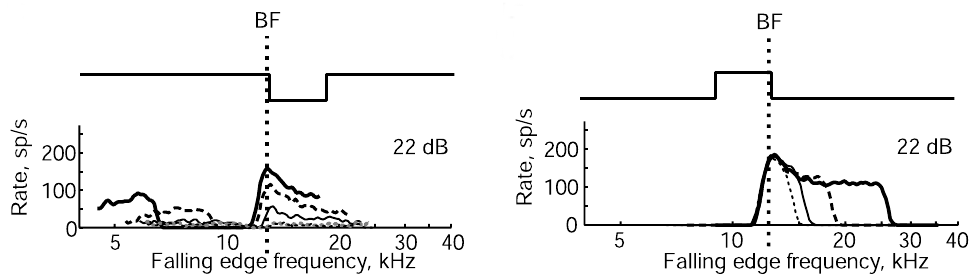
\includegraphics{TV_Notch/Reiss_Fig9_E+F.eps}}\\
  \resizebox{\textwidth}{!}{\includegraphics{TV_Notch/Reiss_Fig10A+B.eps}}
  \resizebox{\textwidth}{!}{\includegraphics[height=\textwidth,keepaspectratio,angle=-90]{TV_Notch/Best-Offset2/BestSweep.eps}}\\
  \caption[Response of optimised TV cell (CF=12.76~kHz) to notch and band   sweeps]{Response of optimised TV cell (CF=12.76~kHz) to notch and band sweeps with stimulus sound level at 50 dB SPL\@.
Mean rate responses are plotted against the rising edge frequency of the notch and falling edge of the band-pass in octaves relative to 12.7~kHz. 
Middle row is from Figure 9 E and F in Reiss and Young, second bottom row is from Figure 10 A and B. }   \label{fig:TV_SweepUnit70}
\end{figure}



% \begin{figure}[h!]
%   \centering
% %   \resizebox{\textwidth}{!}{\includegraphics{NoFigure}}
%   \resizebox{\textwidth}{!}{\includegraphics[height=\textwidth,keepaspectratio,angle=-90]{./TV_Notch/Best-Offset2/BestSweep.eps}}\\
%   \caption{Response of TV cell (CF=12.76~kHz, with optimised parameters except
%   offset) and DS cell to half octave notch and band sweeps with stimulus sound
%   level at 50 dB SPL\@. Mean rate responses are plotted against the rising
%   edge frequency of the notch and falling edge of the band-pass in octaves
%   relative to 12.7~kHz.}
%   \label{fig:TV_SweepUnit}
% \end{figure}


% \subsection{Tone Response}
% \begin{figure}[h!]
%   \centering\resizebox{0.95\textwidth}{!}{%
%   \includegraphics{RateLevel/psthsingle90.1.eps}%
%   \includegraphics{RateLevel/TV_ratelevel.eps}}
% \end{figure}
% \begin{figure}[h!]
%   \centering\resizebox{0.95\textwidth}{!}{%
%   \includegraphics{RateLevel/response_area.1.eps}%
%   \includegraphics{RateLevel/response_area_log2.1.eps}}
% \end{figure}
% \begin{figure}[h!]
%   \centering\resizebox{0.95\textwidth}{!}{%
% %   \includegraphics{RateLevel/response_area.1.eps}
%   \includegraphics{RateLevel/psthall90.1.eps}%
%   \includegraphics{RateLevel/psthVlevel.1.eps}}
% \end{figure}


% \clearpage
% \subsection{Noise Response}
% \begin{figure}[h!]
%   \centering\resizebox{0.95\textwidth}{!}{%
%   \includegraphics{NoiseRateLevel/psthsingle120.1.eps}%
%   \includegraphics{NoiseRateLevel/TV_ratelevel.eps}}
% \end{figure}
% \begin{figure}[h!]
%   \centering\resizebox{0.95\textwidth}{!}{%
%   \includegraphics{NoiseRateLevel/response_area.1.eps}%
%   \includegraphics{NoiseRateLevel/response_area_log2.1.eps}}
% \end{figure}
% \begin{figure}[h!]
%   \centering\resizebox{0.95\textwidth}{!}{%
% %   \includegraphics{RateLevel/response_area.1.eps}
%   \includegraphics{NoiseRateLevel/psthall90.1.eps}%
%   \includegraphics{NoiseRateLevel/psthVlevel.1.eps}}
% \end{figure}


% \clearpage
% \subsection{Masked Noise and Tone}
% \begin{figure}[h!]
%   \centering\resizebox{0.95\textwidth}{!}{\includegraphics{MaskedRateLevel/psthsingle90.1.eps}\includegraphics{MaskedRateLevel/TV_ratelevel.eps}}
% \end{figure}
% \begin{figure}[h!]
%   \centering\resizebox{0.95\textwidth}{!}{%
%   \includegraphics{MaskedRateLevel/response_area.1.eps}%
%   \includegraphics{MaskedRateLevel/response_area_log2.1.eps}}
% \end{figure}
% \begin{figure}[h!]
%   \centering\resizebox{0.95\textwidth}{!}{%
% %   \includegraphics{RateLevel/response_area.1.eps}
%   \includegraphics{MaskedRateLevel/psthall90.1.eps}%
%   \includegraphics{MaskedRateLevel/psthVlevel.1.eps}}
% \end{figure}
% \clearpage
% \subsection{Masked Response Area}
% \begin{figure}[h!]
%   \centering\resizebox{0.95\textwidth}{!}{%
%   \includegraphics{MaskedResponseCurve/psthsingle5810.1.eps}%
%   \includegraphics{MaskedResponseCurve/TV_masked.eps}}
% \end{figure}
% \begin{figure}[h!]
%   \centering\resizebox{0.95\textwidth}{!}{%
%   \includegraphics{MaskedResponseCurve/response_area.1.eps}%
%   \includegraphics{MaskedResponseCurve/response_area_log2log2.1.eps}}
% \end{figure}
% \begin{figure}[h!]
%   \centering\resizebox{0.95\textwidth}{!}{%
% %   \includegraphics{RateLevel/response_area.1.eps}
%   \includegraphics{MaskedResponseCurve/psthall5810.1.eps}%
%   \includegraphics{MaskedResponseCurve/psthVmod.1.eps}}
% \end{figure}
% \clearpage






 


%%% Local Variables: 
%%% mode: latex
%%% mode: tex-fold
%%% TeX-master: "SimpleResponses"
%%% TeX-PDF-mode: nil
%%% End: 
